\documentclass[tikz, convert={outext=.svg,pdf2svg}]{standalone}

\usepackage{tikz,amsmath, amssymb,bm,color}
\usetikzlibrary{shapes,arrows}
\usetikzlibrary{calc}

\definecolor{myblue}{RGB}{175, 204, 233}

\begin{document}
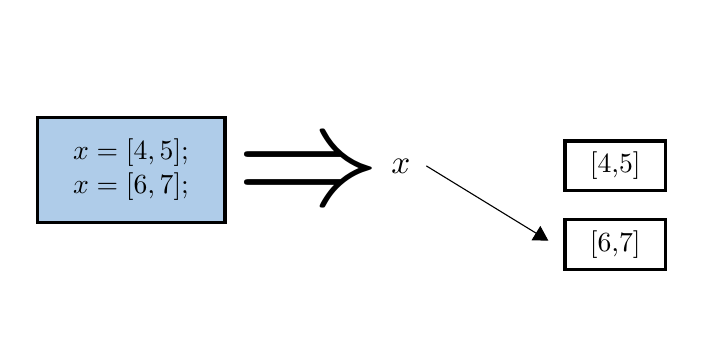
\begin{tikzpicture}

\tikzstyle{square} = [draw,outer sep=7,inner sep=3,minimum size=10,line width=1, 
very thick, draw=black!100, top color=white,bottom color=white]
\tikzstyle{white-b} = [draw,outer sep=7,inner sep=7,minimum size=20,line width=1, 
very thick, draw=blue!25, top color=blue!25, bottom color=blue!25]
\tikzstyle{gray-b} = [draw,outer sep=7,inner sep=7,minimum size=20,line width=1, 
very thick, draw=black!100, top color=myblue, bottom color=myblue]
\tikzstyle{black_block} = [draw, text=white, font=\bf
, outer sep=7,inner sep=5,minimum size=20,line width=1,
very thick, draw=black!5, top color=black!50,bottom color=black]
\tikzstyle{gray_block}= [draw,outer sep=7,inner sep=3,minimum size=20,line width=1,very thick, draw=black!95, top color=white,bottom color=blue!25];
\tikzstyle{red_block}= [draw,outer sep=7,inner sep=3,minimum size=20,line width=1,very thick, draw=red!95, top color=white,bottom color=red!25];


\node [gray-b] at (8,15.5) {\begin{tabular}{c} $x=[4,5]$;\\ $x=[6,7];$\end{tabular}};

\node[anchor=center,scale=5.2] at (10.25,15.5) {\begin{tabular}{l} $\Rightarrow$ \end{tabular}}; 
\node[anchor=east,scale=1.2] at (11.95,15.55) {\begin{tabular}{l} $x$ \end{tabular}}; 


%\draw[-triangle 60]  (11.75,15.55) -- (13.25,16);
\draw[-triangle 60]  (11.75,15.55) -- (13.3,14.6);

\node [square, anchor=center] at (14.15,15.55) {\begin{tabular}{c} [4,5]\end{tabular}};
\node [square, anchor=center] at (14.15,14.55) {\begin{tabular}{c} [6,7]\end{tabular}};





\phantom{
%\draw[dashed,color=red!80!black,thick,fill=red!80!black, opacity=0.2] (7.5,14.7) rectangle (12.95,13.05);
%\draw[dashed,color=red!80!black,thick,fill=red!80!black, opacity=0.2] (7.5,12.2) rectangle (12.7,10.55);
}





\usetikzlibrary{calc}
\pgftransformreset
\node[inner sep=0pt,outer sep=0pt,minimum size=0pt,line width=0pt,text width=0pt,text height=0pt] at (current bounding box) {};
%add border to avoid cropping by pdflibnet
\foreach \border in {0.1}
  \useasboundingbox (current bounding box.south west)+(-\border,-\border) rectangle (current bounding box.north east)+(\border,\border);
\newwrite\metadatafile
\immediate\openout\metadatafile=\jobname_BB.txt
\path
  let
    \p1=(current bounding box.south west),
    \p2=(current bounding box.north east)
  in
  node[inner sep=0pt,outer sep=0pt,minimum size=0pt,line width=0pt,text width=0pt,text height=0pt,draw=white] at (current bounding box) {
\immediate\write\metadatafile{\p1,\p2}
};
\immediate\closeout\metadatafile
\end{tikzpicture}

\end{document}


